\documentclass[handout,12pt,dvipsnames,t]{beamer}
\setbeamertemplate{footline}[frame number]
\title{Statistical Practice in Epidemiology \newline }
\subtitle{Poisson and Logistic Regression} % \\[10mm]
\author{Janne Pitk\"aniemi (EL) }
\date{}

\usepackage{listings}
\usepackage{color}

%\definecolor{dkgreen}{rgb}{0,0.6,0}
%\definecolor{gray}{rgb}{0.5,0.5,0.5}
%\definecolor{mauve}{rgb}{0.58,0,0.82}
\lstset{frame=NA,
language=R,
aboveskip=3mm,
belowskip=3mm,
showstringspaces=false,
columns=flexible,
numbers=none,
% keywordstyle=\color{RoyalBlue},
% numberstyle=\tiny\color{gray},
% commentstyle=\color{dkgreen},
% stringstyle=\color{mauve},
breaklines=true,
breakatwhitespace=true,
tabsize=3,
keywords={}
}
\usepackage{Sweave}
\begin{document}
\lstset{basicstyle=\footnotesize}




\maketitle
\Sconcordance{concordance:SPE-Poisson-Logistic-Regression.tex:SPE-Poisson-Logistic-Regression.Rnw:%
1 29 1 1 0 3 1 1 3 376 1 1 18 11 0 1 2 27 1 1 2 1 0 4 1 3 0 1 2 73 1 1 %
2 1 0 1 1 1 2 7 1 17 0 1 2 6 1 1 2 1 0 1 1 1 5 3 0 1 1 15 0 1 2 120 1 1 %
2 1 0 1 1 6 0 1 2 4 1 1 2 1 0 1 1 3 0 1 2 4 1 1 2 7 0 1 2 4 1 1 2 7 0 1 %
2 8 1 1 2 1 0 3 1 6 0 1 2 5 1 1 2 1 0 4 1 8 0 1 2 20 1}




\begin{frame}[fragile]
\frametitle{Points to be covered}

\begin{itemize}
\item Incidence rates, rate ratios and rate differences from\\ {\it follow-up studies}
 can be computed by fitting {\it Poisson regression models}.
\item Odds ratios can be computed from binary data by fitting \\ {\it Logistic regression models}.
\item Odds-ratios can be estimated from case-control studies.
\item Both models are special instances of \\
{\it Generalized linear models}.
\item There are various ways to do these tasks in R.
\end{itemize}

\end{frame}

%----------------------------------------------------------------------
\begin{frame}
\frametitle{The Estonian Biobank cohort: survival among the elderly}
Follow-up of 60 random individuals aged 75-103 at recruitment, until death ($\bullet$) or censoring (o) in April 2014 (linkage with the Estonian Causes of Death Registry). \\[-0.5cm]
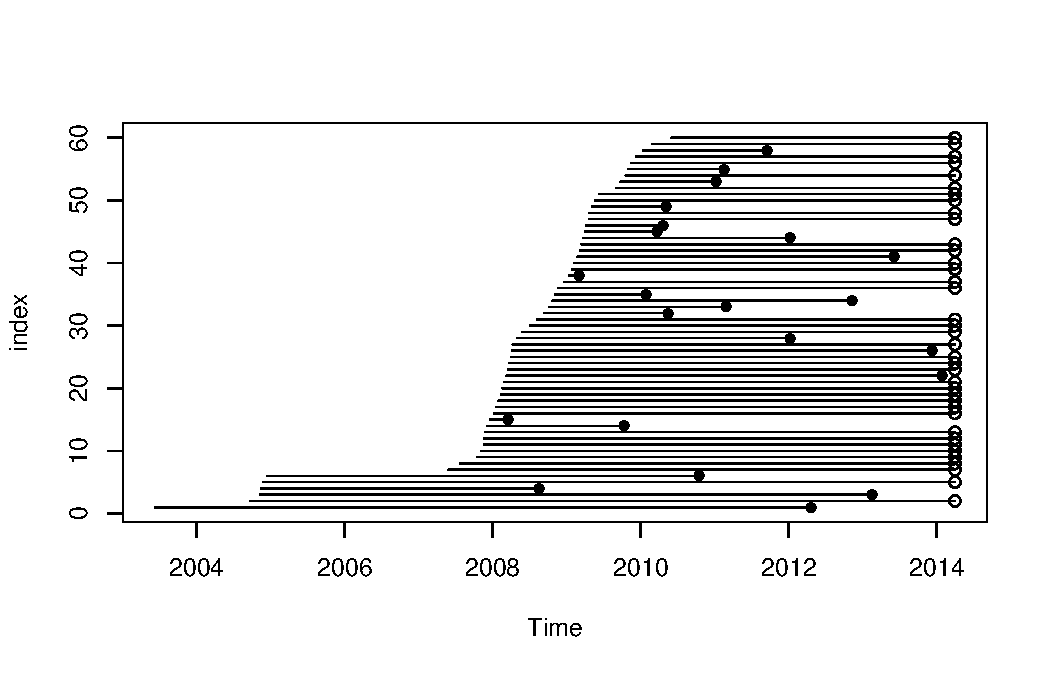
\includegraphics[height=6.5cm]{over75lines}
\end{frame}

%----------------------------------------------------------------------
\begin{frame}
\frametitle{The Estonian Biobank cohort: survival among the elderly}
Follow-up time for 60 random individuals aged 75-103 at recruitment (time-scale: time in study). \\[-0.5cm]
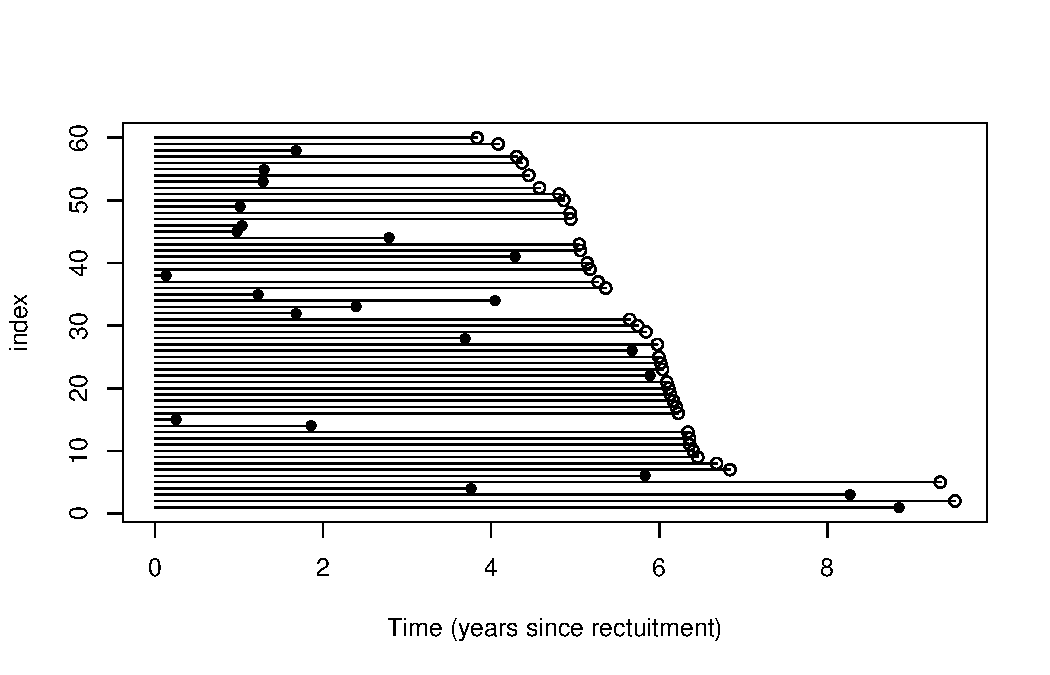
\includegraphics[height=6.5cm]{over75fulines}
\end{frame}

\begin{frame}
\frametitle{Events, dates and risk time}
\begin{itemize} %[<+->]
\item Mortality as the outcome:
\begin{description}
  \item[\tt d:] indicator for {\bf status} at exit: \\
        {\bf 1}: death observed \\
        {\bf 0}: censored alive
\end{description}
\item Dates:
  \begin{align*}
    \texttt{doe} & = \text{date of {\bf E}ntry to follow-up}, \\
    \texttt{dox} & = \text{date of e{\bf X}it, end of follow-up}.
  \end{align*}
\item Follow-up time (years) computed as:
\[
\mathtt{y}= \mbox{\tt (dox - doe)/365.25}
\]
\end{itemize}
\end{frame}


\begin{frame}[fragile]
\frametitle{Crude overall rate computed in two ways}

Total no. cases, person-years \& rate (/1000 y):
\small
\begin{lstlisting}
>  D <- sum( d ); Y <- sum(y) ; R <- D/(Y/1000)
>   round( c(D=D, Y=Y, R=R), 2)
   D      Y         R 
  884.00 11678.24    75.70 
\end{lstlisting}
%\pause
\normalsize
Poisson regression model with only intercept
(``{\tt 1}'').
\small
\begin{lstlisting}
> m1 <- glm( d ~ 1, family=poisson, offset=log(y))
> coef(m1)
(Intercept) 
  -2.581025 

> exp( coef(m1) )*1000
(Intercept) 
   75.69636 
\end{lstlisting}
\normalsize
\emph{Why do we get the same results?}
\end{frame}

%----------------------------------------------------------------------
\begin{frame}[fragile]
\frametitle{Constant hazard --- Poisson model}

Let $Y\sim exp(\lambda)$, then $f(y;\lambda)=\lambda e^{-\lambda y} I(y > 0 )$

Constant rate: $\lambda(y)=\frac{f(y;\lambda)}{S(y;\lambda)}=\lambda$

Observed data $ \left\{ (y_i,\delta_i); i=1,...,n \right\}$.

The likelihood \vspace*{0.2in} $L(\lambda)=\prod_{i=1}^{n} \lambda^{\delta_i} e^{-\lambda y_i}$ and $log(L)= \sum_{i=1}^{n} \left[  \delta_i log(\lambda)-\lambda y_i \right]$

Solving the {\it score equations}: \ $\frac{\partial \log L(\lambda)}{\partial \lambda} = \sum \left[  \frac{\delta_i}{\lambda} -y_i \right] $ \\ %\vspace*{0.2in}
 $=  \frac{D}{\lambda} - Y = 0 $ and $  D-\lambda Y   =  0   $

$\rightarrow$
{\bf maximum likelihood estimator} (MLE) of $\lambda$:
$$
 \widehat\lambda = \frac{D}{Y}  =
  \frac{\mbox{number of cases}}
  {\mbox{total person-time}}
  = \mbox{ empirical rate!}
$$
\end{frame}

%----------------------------------------------------------------------
\begin{frame}[fragile]
\frametitle{offset term --- Poisson model}

\begin{itemize}
\item Previous model without offset: Intercept 6.784=log(884)

\item We should use an offset if we suspect that the
underlying \textbf{population sizes (person-years) differ }
for each of the observed counts -- For example varying person-years by tratment group, sex,age,... 

\item We need a term in the model that "scales" the likelihood, but does not depend on model parameters ( include a \textbf{term with reg. coef. fixed to 1}) -- offset term is log(y)
\end{itemize}

\begin{center}
$log(\frac{\mu}{y})=\beta_0+\beta_1 x_1$ \\
$log(\mu)=1 \times log(y)+\beta_0+\beta_1 x_1$
\end{center}
\end{frame}

%----------------------------------------------------------------------
\begin{frame}[fragile]
\frametitle{Comparing rates: The Thorotrast Study}
\begin{itemize}
\item
Cohort of seriously ill patients in Denmark
on whom angiography of brain was performed.
\vspace{\medskipamount}
\item
Exposure: {\tt contrast} medium used in angiography,
\begin{enumerate}
\item {\tt thor} = thorotrast (with $^{232}$Th), used 1935-50
\item {\tt ctrl} = other medium (?), used 1946-63
\end{enumerate}
\item
Outcome of interest: death
  \begin{align*}
    \texttt{doe} & = \text{date of {\bf E}ntry to follow-up}, \\
    \texttt{dox} & = \text{date of e{\bf X}it, end of follow-up}.
  \end{align*}
\item {\tt data(thoro)} in the {\tt Epi} package.
\end{itemize}
\end{frame}

%----------------------------------------------------------------------
\begin{frame}[fragile]
\frametitle{Comparing rates: thorotrast vs. control}
Tabulating cases, person-years \& rates by group

\lstset{basicstyle=\footnotesize}
\begin{lstlisting}
> stat.table( contrast,
+             list( N = count(),
+                   D = sum(d),
+                   Y = sum(y),
+                rate = ratio(d,y,1000) ) )
 --------------------------------------------
 contrast         N       D        Y    rate
 --------------------------------------------
  ctrl         1236  797.00 30517.56   26.12
  thor          807  748.00 19243.85   38.87
 --------------------------------------------
\end{lstlisting}
\normalsize
Rate ratio, RR = $38.89/26.12 = 1.49$, \\
Std. error of log-RR, SE  = $\sqrt{1/748 + 1/797} = 0.051$, \\
Error factor, EF = $\exp(1.96 \times 0.051) = 1.105$, \\
95\% confidence interval for RR:\\
$(1.49/1.105, 1.49\times 1.105) =
 (1.35, 1.64)$.
\end{frame}


\begin{frame}[fragile]
\frametitle{Rate ratio estimation with Poisson regression}
\begin{itemize}
\item Include {\tt contrast} as the explanatory variable (factor).
\item Insert person years in units that you want rates in
\lstset{basicstyle=\footnotesize}
\begin{lstlisting}
> m2 <- glm( d ~ contrast, offset=log(y/1000),
+                family = poisson )
> round( summary(m2)$coef, 4)[, 1:2]

              Estimate Std. Error
(Intercept)     3.2626     0.0354
contrast thor   0.3977     0.0509
\end{lstlisting}
\normalsize
\item Rate ratio and CI?\\
Call function {\tt ci.exp()} in {\tt Epi}
\lstset{basicstyle=\ttfamily\footnotesize}
\begin{lstlisting}
> round( ci.exp( m2 ), 3 )

              exp(Est.)   2.5%  97.5%
(Intercept)      26.116 24.364 27.994
contrast thor     1.488  1.347  1.644
\end{lstlisting}
\normalsize
\end{itemize}
\end{frame}

\begin{frame}[fragile]
\frametitle{Rates in groups with Poisson regression}

\begin{itemize} %[<+->]
\item Include {\tt contrast} as the explanatory variable (factor).
\item Remove the intercept (\texttt{-1})
\item Insert person-years in units that you want rates in
\lstset{basicstyle=\ttfamily\footnotesize}
\begin{lstlisting}
> m3 <- glm( d ~ contrast - 1, 
                 offset=log(y/1000),
+                family = poisson )
> round( summary(m3)$coef, 4)[, 1:2]

              Estimate Std. Error
contrast ctrl   3.2626     0.0354
contrast thor   3.6602     0.0366

> round( ci.exp( m3 ), 3 )

              exp(Est.)   2.5%  97.5%
contrast ctrl    26.116 24.364 27.994
contrast thor    38.870 36.181 41.757
\end{lstlisting}
\normalsize
\end{itemize}
\end{frame}

%----------------------------------------------------------------------
\begin{frame}[fragile]
\frametitle{Rates in groups with Poisson regression}
\begin{itemize}[<+->]
\item You can have it all in one go:
\lstset{basicstyle=\ttfamily\footnotesize}
\begin{lstlisting}
> CM <- rbind( c(1,0), c(0,1), c(-1,1) )
> rownames(CM) <- c("Ctrl","Thoro","Th vs.Ct")
> colnames(CM) <- names( coef(m3) )
> CM
          contrast ctrl contrast thor
Ctrl                  1             0
Thoro                 0             1
Th vs. Ct            -1             1
\end{lstlisting}

\begin{lstlisting}
> round( ci.exp( m3, ctr.mat=CM ),3 )
\end{lstlisting}
\begin{lstlisting}
          exp(Est.)   2.5%  97.5%
Ctrl         26.116 24.364 27.994
Thoro        38.870 36.181 41.757
Th vs. Ct     1.488  1.347  1.644
\end{lstlisting}
\normalsize
\end{itemize}
\end{frame}

%----------------------------------------------------------------------
\begin{frame}[fragile]
\frametitle{Rate ratio estimation with Poisson regression}

\begin{itemize}
\item Response may also be specified as individual {\it rates}:\\
{\tt d/y} \\
{\tt weights=} instead of {\tt offset=} are needed.
\lstset{basicstyle=\ttfamily\footnotesize}
\begin{lstlisting}
> m4<-glm( d/(y/1000)~contrast, weights=y/1000,
+            family=poisson)
> round( ci.exp(m4), 3 )
\end{lstlisting}
\begin{lstlisting}
              exp(Est.)   2.5%  97.5%
(Intercept)      26.116 24.365 27.994
contrast thor     1.488  1.347  1.644
\end{lstlisting}
\normalsize
\end{itemize}
\end{frame}


%----------------------------------------------------------------------
\begin{frame}[fragile]
\frametitle{Rate difference estimation with Poisson regression}

\begin{itemize}
\item The approach with \texttt{d/y} enables additive rate models too:
\lstset{basicstyle=\ttfamily\footnotesize}
\begin{lstlisting}
> m5 <-glm(d/(y/1000) ~contrast,weights=y/1000,
+            family=poisson(link="identity") )
> round( ci.exp(m5,Exp=F), 3 )
\end{lstlisting}
\begin{lstlisting}
              Estimate   2.5%  97.5%
(Intercept)     26.116 24.303 27.929
contrast thor   12.753  9.430 16.077
\end{lstlisting}
\end{itemize}
\end{frame}

%----------------------------------------------------------------------
\begin{frame}[fragile]
\frametitle{Rates difference}
\begin{itemize}
\item As before you can have it all:
\lstset{basicstyle=\ttfamily\footnotesize}
\begin{lstlisting}
> m6 <- glm( d/(y/1000) ~ contrast -1,
+  family = poisson(link="identity"), 
+  weights = y/1000)
> round(ci.exp(m6, ctr.mat=CM, Exp=F ), 3)
\end{lstlisting}
\begin{lstlisting}
          Estimate   2.5%  97.5%
Ctrl        26.116 24.303 27.929
Thoro       38.870 36.084 41.655
Th vs. Ct   12.753  9.430 16.077
\end{lstlisting}
\begin{lstlisting}
> round( ci.exp( m3, ctr.mat=CM), 3 )
\end{lstlisting}
\begin{lstlisting}
          exp(Est.)   2.5%  97.5%
Ctrl         26.116 24.364 27.994
Thoro        38.870 36.181 41.757
Th vs. Ct     1.488  1.347  1.644
\end{lstlisting}
\normalsize
\end{itemize}
\end{frame}

%----------------------------------------------------------------------
\begin{frame}[fragile]
\frametitle{Binary data: Treatment success Y/N}
85 diabetes-patients with foot-wounds:
\begin{itemize}
\item Dalterapin (Dal)
\item Placebo (Pl)
\end{itemize}

Treatment/Placebo given to diabetes patients, the design is
propective because outcome is measured better/worse. Is the probability of outcome more than 15\% -- yes, then use the risk difference or risk ratio (RR) 

%\begin{center}
%\begin{tabular}{rcc}
%\toprule
%   & \multicolumn{2}{c}{Treatment group} \\
%\cmidrule{2-3}
%     & Dalterapin & Placebo \\
%\midrule
%Outcome:\hspace*{1em} Better & 29 & 20 \\
%                     Worse  & 14 & 22 \\
%\midrule
%    & 43 & 42 \\
%\bottomrule
%\end{tabular}\\
%\end{center}

\begin{center}
\begin{tabular}{l|r|r}
\hline
\multicolumn{1}{c|}{ } & \multicolumn{2}{|c}{Treatment group} \\
\cline{2-3}
  & Dalterapin & Placebo\\
\hline
Better & 29 & 20\\
\hline
Worse & 14 & 22\\
\hline
Total & 43 & 42\\
\hline
\end{tabular}\end{center}

\[
\hat p_\text{Dal} = \frac{29}{43} = 67\% \qquad
\hat p_\text{Pl}  = \frac{20}{42} = 47\%
\]

\end{frame}

%----------------------------------------------------------------------
\begin{frame}[fragile]
The difference between the probabilities is the fraction of the
patients that benefit from the treatment: $ p_\text{Dal}- p_\text{Pl}$
% \begin{eqnarray*}
% \hat p_\text{Dal} -
% \hat p_\text{Pl} & = & 20\% \\ \\
% \se(\hat p_\text{Dal} - \hat p_\text{Pl}) & = &
%  \sqrt{
%  \frac{p_\text{Dal}(1-p_\text{Dal})}
%       {n_\text{Dal}} +
%  \frac{p_\text{Pl}(1-p_\text{Pl})}
%       {n_\text{Pl}} } \\ & = & 0.11 \\ \\
% 95\% \text{c.i.} & : & 20\% \pm 1.96 \times 11\% = ( 0\%;  40\% )
% \end{eqnarray*}

%\lstset{basicstyle=\ttfamily\scriptsize}

\begin{footnotesize}
\begin{Schunk}
\begin{Sinput}
> library(Epi)
> dlt <- rbind( c(29,14), c(20,22) )
> colnames( dlt ) <- c("Better","Worse")
> rownames( dlt ) <- c("Dal","Pl")
> kable(twoby2( dlt ),"latex")
\end{Sinput}
\end{Schunk}
\end{footnotesize}


\begin{footnotesize}
\begin{lstlisting}
2 by 2 table analysis:
/.../
    Better Worse    P(Better) 95% conf. interval
Dal     29    14       0.6744    0.5226   0.7967
Pl      20    22       0.4762    0.3316   0.6249

                                   95% conf. interval
             Relative Risk: 1.4163    0.9694   2.0692
         Sample Odds Ratio: 2.2786    0.9456   5.4907
Conditional MLE Odds Ratio: 2.2560    0.8675   6.0405
    Probability difference: 0.1982   -0.0110   0.3850

             Exact P-value: 0.0808
        Asymptotic P-value: 0.0665
\end{lstlisting}
\end{footnotesize}
\normalsize
\end{frame}

\begin{frame}[fragile]
  \frametitle{Logistic regression for binary data}
  For grouped binary data, the response is a two-column matrix with
  columns (successes,failures).

% \begin{lstlisting}
% > trt <- factor(c("Dal","Pl"))
% > b1 <- glm( dlt ~ trt, family=binomial )
% > ci.exp( b1 )
% \end{lstlisting}
% \begin{lstlisting}
%             exp(Est.)      2.5%    97.5%
% (Intercept) 2.0714286 1.0945983 3.919992
% trtPl       0.4388715 0.1821255 1.057557
% \end{lstlisting}
% Oops! Dalterapin has become the reference group; we want Placebo to be
% the reference\ldots
% \end{frame}

%----------------------------------------------------------------------
%\begin{frame}[fragile]
%  \frametitle{Logistic regression for binary data}

\begin{lstlisting}
trt <- factor(c("Dal","Pl"))
trt <- relevel( trt, 2 )
b1 <- glm( dlt ~ trt, family=binomial )
round( ci.exp( b1 ), 4 )
\end{lstlisting}
\begin{lstlisting}
            exp(Est.)   2.5%  97.5%
(Intercept)    0.9091 0.4962 1.6657
trtDal         2.2786 0.9456 5.4907
\end{lstlisting}
\begin{itemize}
\item The default parameters in logistic regression are \textbf{odds} (the
intercept: $20/22=0.9090$) and the \textbf{odds-ratio}
($(29/14)/(20/22)=2.28$).

\item This is not what you want, because odds ratio is biased estimate of the
 risk ratio.(recall if p>10\% $\frac{p}{1-p} \not \approx p$)
\end{itemize}

\end{frame}


\begin{frame}[fragile]
\frametitle{Logistic regression for binary data - Risk ratio (Relative risk)}

\footnotesize{
\begin{Schunk}
\begin{Sinput}
> library(Epi)
> library(xtable)
> dlt <- rbind( c(29,14), c(20,22) )
> diab<-expand.grid(dlt)
> colnames(diab)[1]<-"d"
> diab$out <- c("Better","Better","Worse","Worse")
> diab$trt <- as.factor(c("Dal","Pl","Dal","Pl"))
> diab$totals<-rep(rowSums(dlt),2)
> diab$trt<-relevel( diab$trt, 2 )
> print(xtable(diab,digits=c(0,0,0,0,0)),include.rownames = F)
\end{Sinput}
% latex table generated in R 3.5.0 by xtable 1.8-2 package
% Thu Jun 07 10:27:03 2018
\begin{table}[ht]
\centering
\begin{tabular}{rllr}
  \hline
d & out & trt & totals \\ 
  \hline
29 & Better & Dal & 43 \\ 
  20 & Better & Pl & 42 \\ 
  14 & Worse & Dal & 43 \\ 
  22 & Worse & Pl & 42 \\ 
   \hline
\end{tabular}
\end{table}\end{Schunk}
}

\end{frame}

\begin{frame}[fragile]
\frametitle{Logistic regression for binary data - risk ratio}

\begin{Schunk}
\begin{Sinput}
> library(Epi)
> library(xtable)
> b2 <- glm(d/totals~trt, 
+           weights=totals,
+           family=binomial(link="log"),
+           data=diab[c(1,2),])
> xtable(round( ci.exp( b2 ), digits=6 ))
\end{Sinput}
% latex table generated in R 3.5.0 by xtable 1.8-2 package
% Thu Jun 07 10:27:03 2018
\begin{table}[ht]
\centering
\begin{tabular}{rrrr}
  \hline
 & exp(Est.) & 2.5\% & 97.5\% \\ 
  \hline
(Intercept) & 0.48 & 0.35 & 0.65 \\ 
  trtDal & 1.42 & 0.97 & 2.07 \\ 
   \hline
\end{tabular}
\end{table}\end{Schunk}

Diabetics with Dalterapin treatment have 1.4 times the risk of getting better than  
those treated with placebo

\end{frame}

%------------------------------
%----------------------------------------------------------------------
% \begin{frame}[fragile]
% \frametitle{Case-control study: Food-poisoning outbreak}
% 
% \begin{itemize}
% \item An outbreak of acute gastrointestinal illness (AGI) occurred in
%   a psychiatric hospital in Dublin in 1996.
% \item Out of all 423 patients and staff members, 65 were
%   affected during 27 to 31 August, 1996.
% \item 65 cases and 62 randomly selected control subjects were
%   interviewed.
% \item Exposure of interest: chocolate mousse cake.
% \item 47 cases and 5 controls reported having eaten the cake.
% \end{itemize}


%----------------------------------
\begin{frame}[fragile]
\frametitle{Logistic regression in case-control studies}

\begin{itemize}

\item Model for disease occurrence in the target population:
\begin{center}
$ \ln\left[\frac{p}{1-p}\right] = \beta_0 + \beta_1 x_1 + \beta_2 x_2 $
\end{center}

\item Sampling fractions:
  P(inclusion in study $\mid$ control)  =  $s_\text{ctr}$ 
  P(inclusion in study  $\mid$ case)  =  $s_\text{case}$ 

\item  Model for observed case-control data:
  \begin{align*}
 \ln[\mbox{odds ( case | incl.) }]
  & = \ln\left[\frac{p}{1-p}\right] +
      \ln\left[\frac{s_\text{cas}}{s_\text{ctr}}\right] \\ \\
  & =  \left( \ln\left[\frac{s_\text{cas}}{s_\text{ctr}}\right] + \beta_0 \right)
         + \beta_1 x_1 + \beta_2 x_2
  \end{align*}
\end{itemize}
\end{frame}

\begin{frame}[fragile]
  \frametitle{Logistic regression in case-control studies}
  
  Analysis of $P(case | inclusion)$ --- \textit{i.e.} binary
observations:
$$
Y=\left\{ \begin{array}{ll}
          1 \quad \sim & \mbox{case}\\
          0 \quad \sim & \mbox{control}
                    \end{array} \right.
$$
$\ln[\mbox{odds ( case | incl.) }] =
 \left( \ln\left[\frac{s_\text{cas}}{s_\text{ctr}}\right] + \beta_0 \right)
         + \beta_1 x_1 + \beta_2 x_2$
\vspace*{1cm}
\begin{itemize}
\item Effect of covariates is estimated correctly.
\item Intercept is meaningless \newline
\hspace*{0.5cm} depends on $s_\text{cas}$ and $s_\text{ctr}$
  that are often unknown.

\end{itemize}
\end{frame}

\begin{frame}[fragile]
\frametitle{Case-control study: Food-poisoning outbreak}

\begin{itemize} %[<+->]
\item An outbreak of acute gastrointestinal illness (AGI) occurred in
  a psychiatric hospital in Dublin in 1996.
\item Out of all 423 patients and staff members, 65 were
  affected during 27 to 31 August, 1996.
\item 65 cases and 62 randomly selected control subjects were
  interviewed.
\item Exposure of interest: chocolate mousse cake.
\item 47 cases and 5 controls reported having eaten the cake.
\end{itemize}

{\small Ref: \verb|http://www.eurosurveillance.org/ViewArticle.aspx?|}
{\small \verb|ArticleId=188|} -- here original numbers somewhat modified.
\end{frame}

\begin{frame}[fragile]
\frametitle{Outbreak: crude summary of data}

\begin{itemize}
\item Target population information
 \begin{itemize}
  \item N = 423, size of the whole study population
  \item D = 65, no. of cases of AGI
  \item B = 358, no. of non-cases
 \end{itemize}
\item Case-control data
\begin{itemize}
\item  C = 62, no. of controls, random sample from 358 non-cases
\item  f = 62/358 = 0.173, sampling fraction of non-cases
\item  D1 = 47 cases exposed to chocolate mousse
\item  D0 = 18 unexposed cases
\item  C1 = 5 controls exposed to chocolate mousse
\item  C0 = 57 unexposed controls
\end{itemize}
\end{itemize}

%{\small Ref: \verb|http://www.eurosurveillance.org/ViewArticle.aspx?|}
%{\small \verb|ArticleId=188|} -- here original numbers somewhat modified.
\end{frame}

\begin{frame}[fragile]
\frametitle{Outbreak: results of analysis}

Overall incidence proportion (IP) of AGI in the population

\scriptsize{
\begin{Schunk}
\begin{Sinput}
> D <- 65; N <- 423; IP <- D/N 
> round(IP, 3)
\end{Sinput}
\begin{Soutput}
[1] 0.154
\end{Soutput}
\end{Schunk}
}

\normalsize
Analysis of case-control data
\scriptsize{
\begin{Schunk}
\begin{Sinput}
> D1 <- 47; D0 <- D - D1; 
> C <- 62 ; C1 <- 5; C0 <- C - C1
\end{Sinput}
\end{Schunk}
}

\normalsize
Case-control ratios by exposure (not as useful as the following!)
\scriptsize{
\begin{Schunk}
\begin{Sinput}
> round( c( D1/C1, D0/C0 ), 2)
\end{Sinput}
\begin{Soutput}
[1] 9.40 0.32
\end{Soutput}
\end{Schunk}
}
\normalsize
Exposure odds in cases and controls

\scriptsize{
\begin{Schunk}
\begin{Sinput}
> round( c( D1/D0, C1/C0 ), 2)
\end{Sinput}
\begin{Soutput}
[1] 2.61 0.09
\end{Soutput}
\end{Schunk}
}
\end{frame}

\begin{frame}[fragile]
\frametitle{Outbreak: results of analysis}

Estimation of the incidence odds ratio (IOR) = exposure odds ratio 

\scriptsize{
\begin{Schunk}
\begin{Sinput}
> IOR <- (D1/D0)/(C1/C0)
> SE.logIOR <- sqrt(1/D1 + 1/D0 + 1/C1 + 1/C0 )
> CI.IOR <- IOR * exp( c(-1,1)*1.96*SE.logIOR )
> round( c(IOR, SE.logIOR, CI.IOR ), 2)
\end{Sinput}
\begin{Soutput}
[1] 29.77  0.54 10.28 86.21
\end{Soutput}
\end{Schunk}
}

\normalsize
Same with glm model

\scriptsize{
\begin{Schunk}
\begin{Sinput}
> count<-c(D1,D0,C1,C0)
> cc<-c(1,1,0,0)
> exposed<-c(1,0,1,0)
> mousse<-data.frame(cbind(cc,exposed,count))
> ci.exp(glm(cc~exposed,weights=count,family="binomial",data=mousse))
\end{Sinput}
\begin{Soutput}
             exp(Est.)       2.5%      97.5%
(Intercept)  0.3157895  0.1858913  0.5364586
exposed     29.7666667 10.2778305 86.2102603
\end{Soutput}
\end{Schunk}
}
\end{frame}

\begin{frame}
\frametitle{Conclusion: What did we learn?}
\begin{itemize} %[<+->]
\item Poisson regression models.
\item In Poisson models the response can be either:
  \begin{itemize}
    \item case indicator {\tt d} with {\tt offset = log(y)}, or
    \item rate {\tt d/y} with {\tt weights = y}.
  \end{itemize}
\item Both may be fitted on either grouped data, or individual
  records.
\item Binary date can be modeled with odds.
\item Case-control studies:\\
  Odds-ratios can be computed by logistic
  regression models, but \textbf{Intercept} from model is \textbf{meaningless}.
\end{itemize}
\end{frame}
\end{document}
